\section{Technical drawings}
\label{appendix:techdraw}
\begin{figure}[!htb]
    \centering
    \includeinkscape[scale=3]{signaturer}
    \caption{Induction loop signatures as supplied by swarco}
    \label{fig:inductionsignatures}
\end{figure}
\begin{table}[!htb]
    \centering
    \begin{tabular}{|l|l|}\hline
        Regular Expression & Explanation \\\hline
        {[A-B]}[1-2] & Collection of upstream movements on a single road\\\hline
        \textcolor{gray}{[A-B][1-2]}Cy & Bicycle movement modifier\\\hline
        \textcolor{gray}{[A-B][1-2]}[Vv] & Left-turn modifier\\\hline
        \textcolor{gray}{[A-B][1-2]}[Hh] & Right-turn modifier\\\hline
        [A-B][1-2](Cy)?([Hh] | [Vv])? & Non-pedestrian movement strings\\\hline
        [a-b][f-g] & Pedestrian light\\\hline
    \end{tabular}
    \caption{Explanation of traffic movement strings used in later drawing. Occasionally the movements seem aggregated in the drawing, e.g. B1+B1h; this does not mean that they follow the same light, but rather that multiple lights share the same approximate physical location.}
    \label{tab:intersectionmovements}
\end{table}
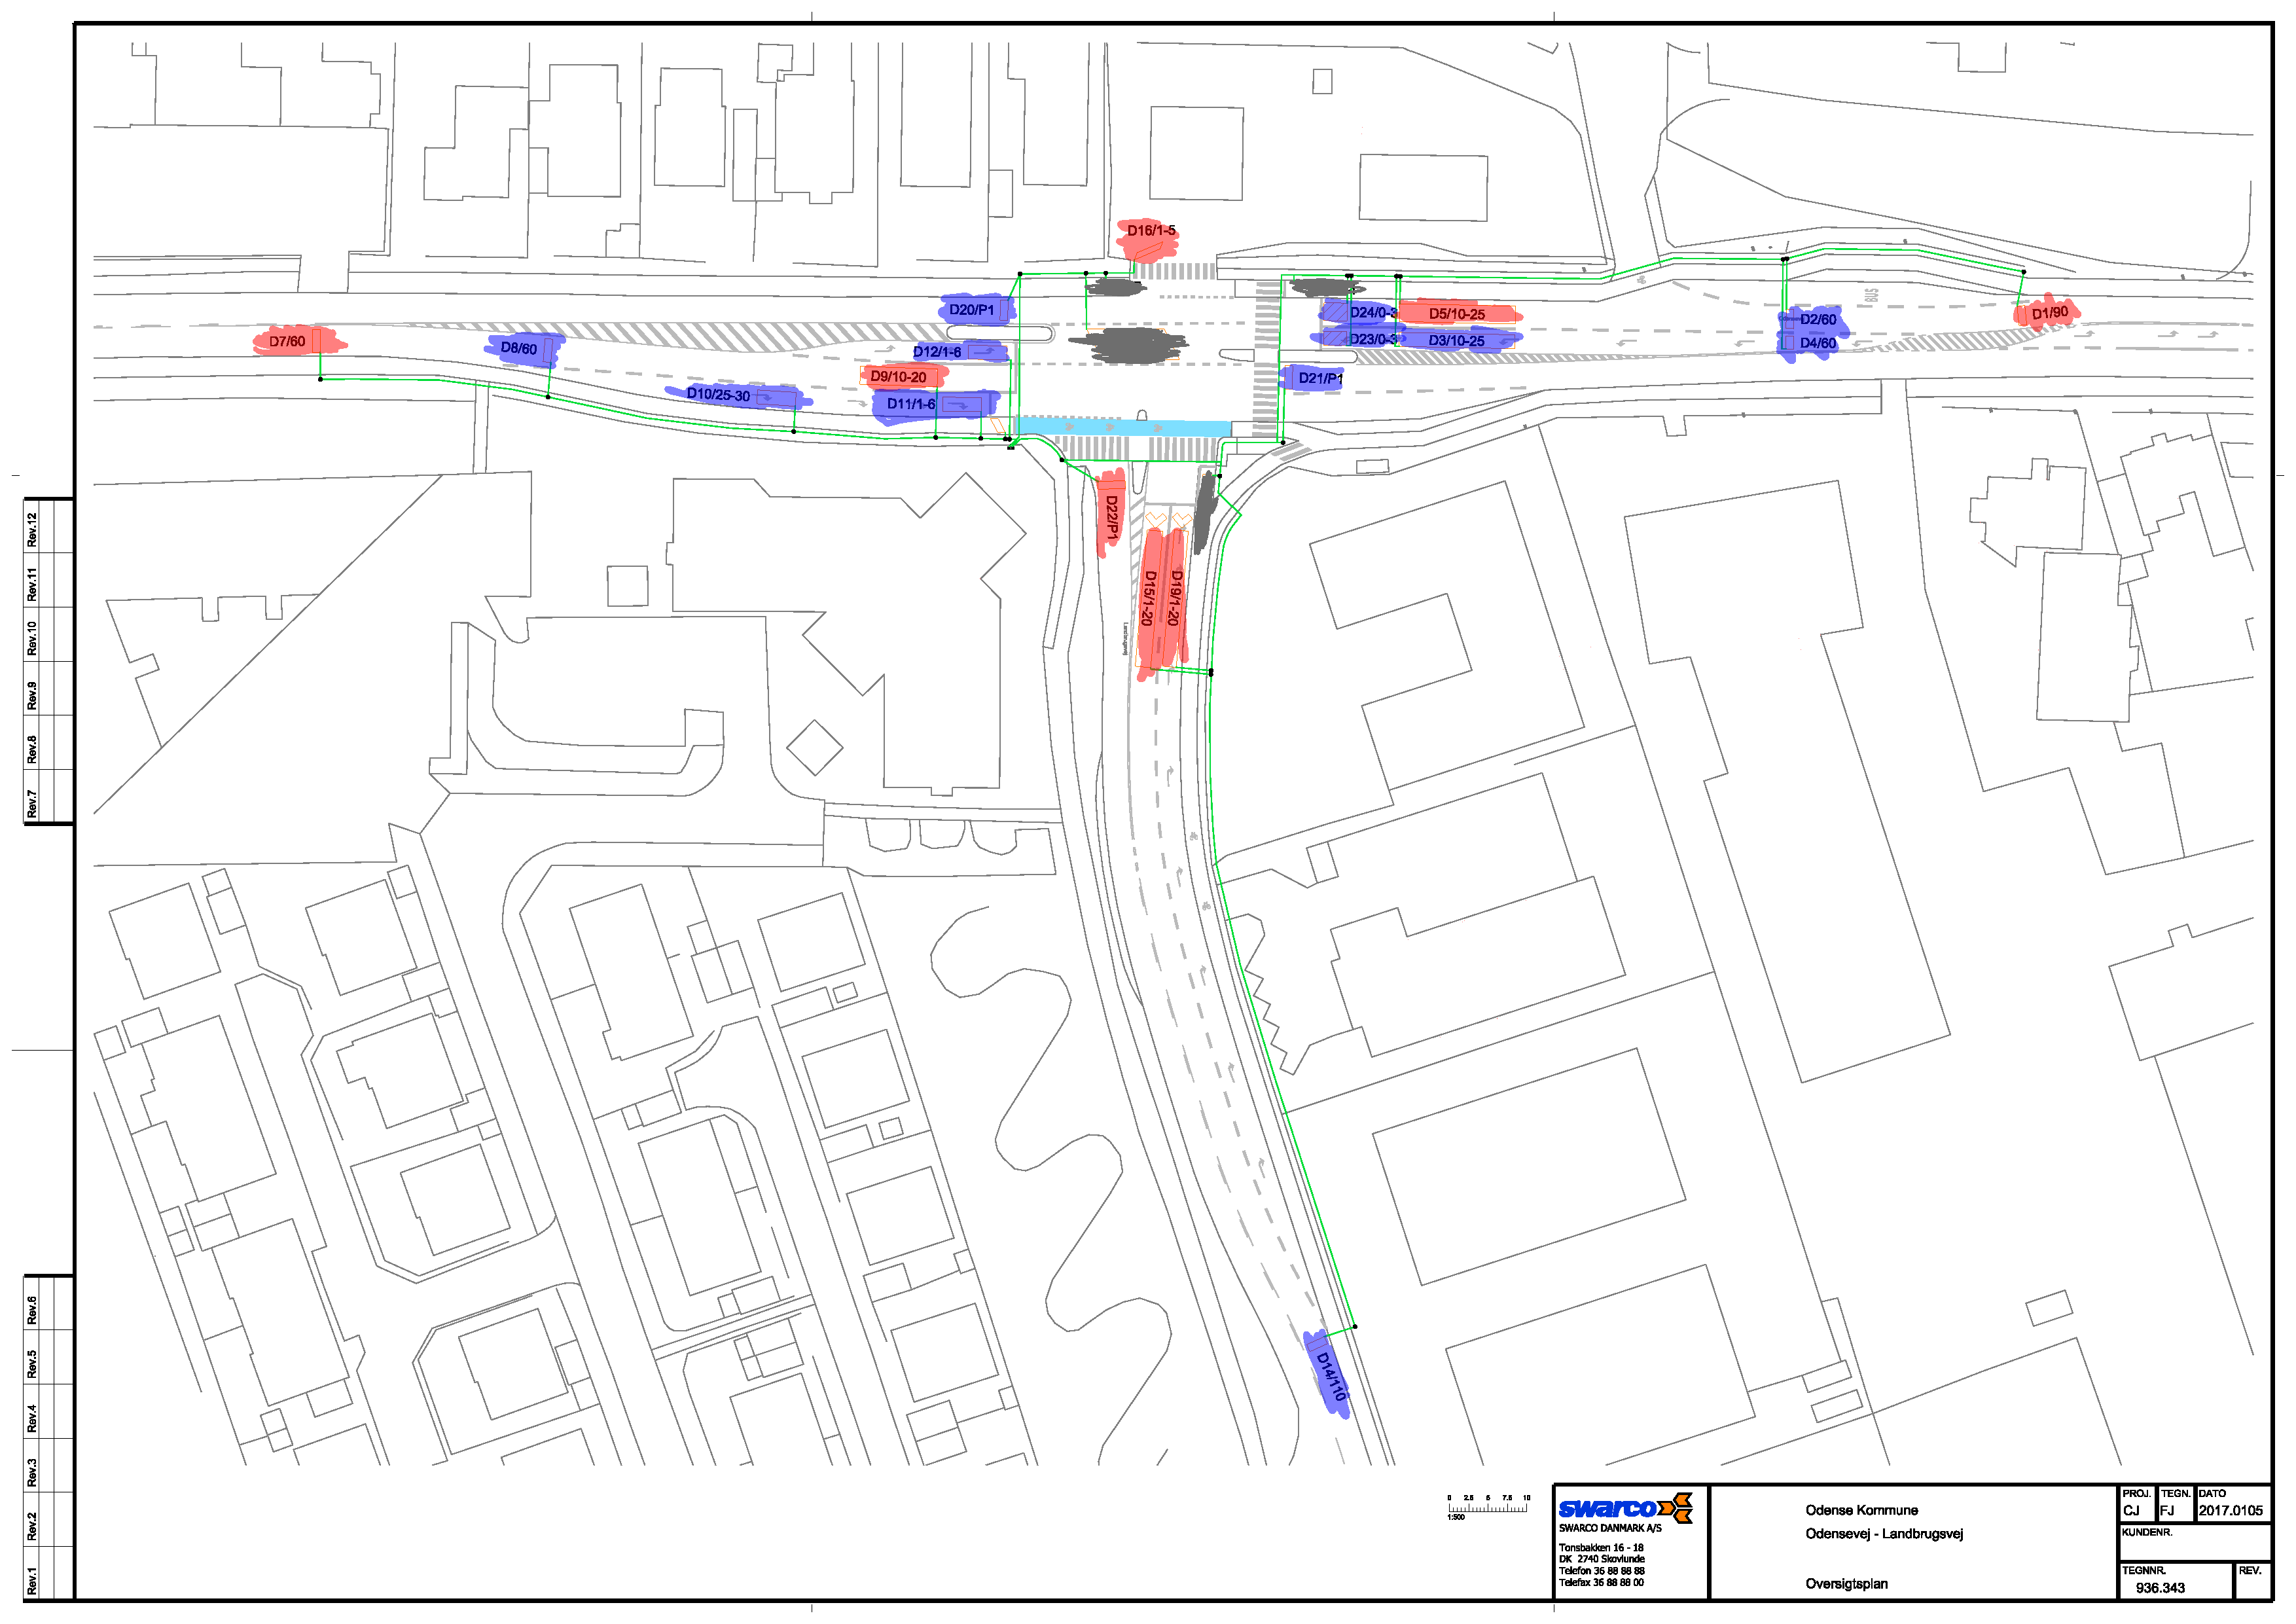
\includepdf[angle=270]{../include/Anl-427-induction-loop.pdf}
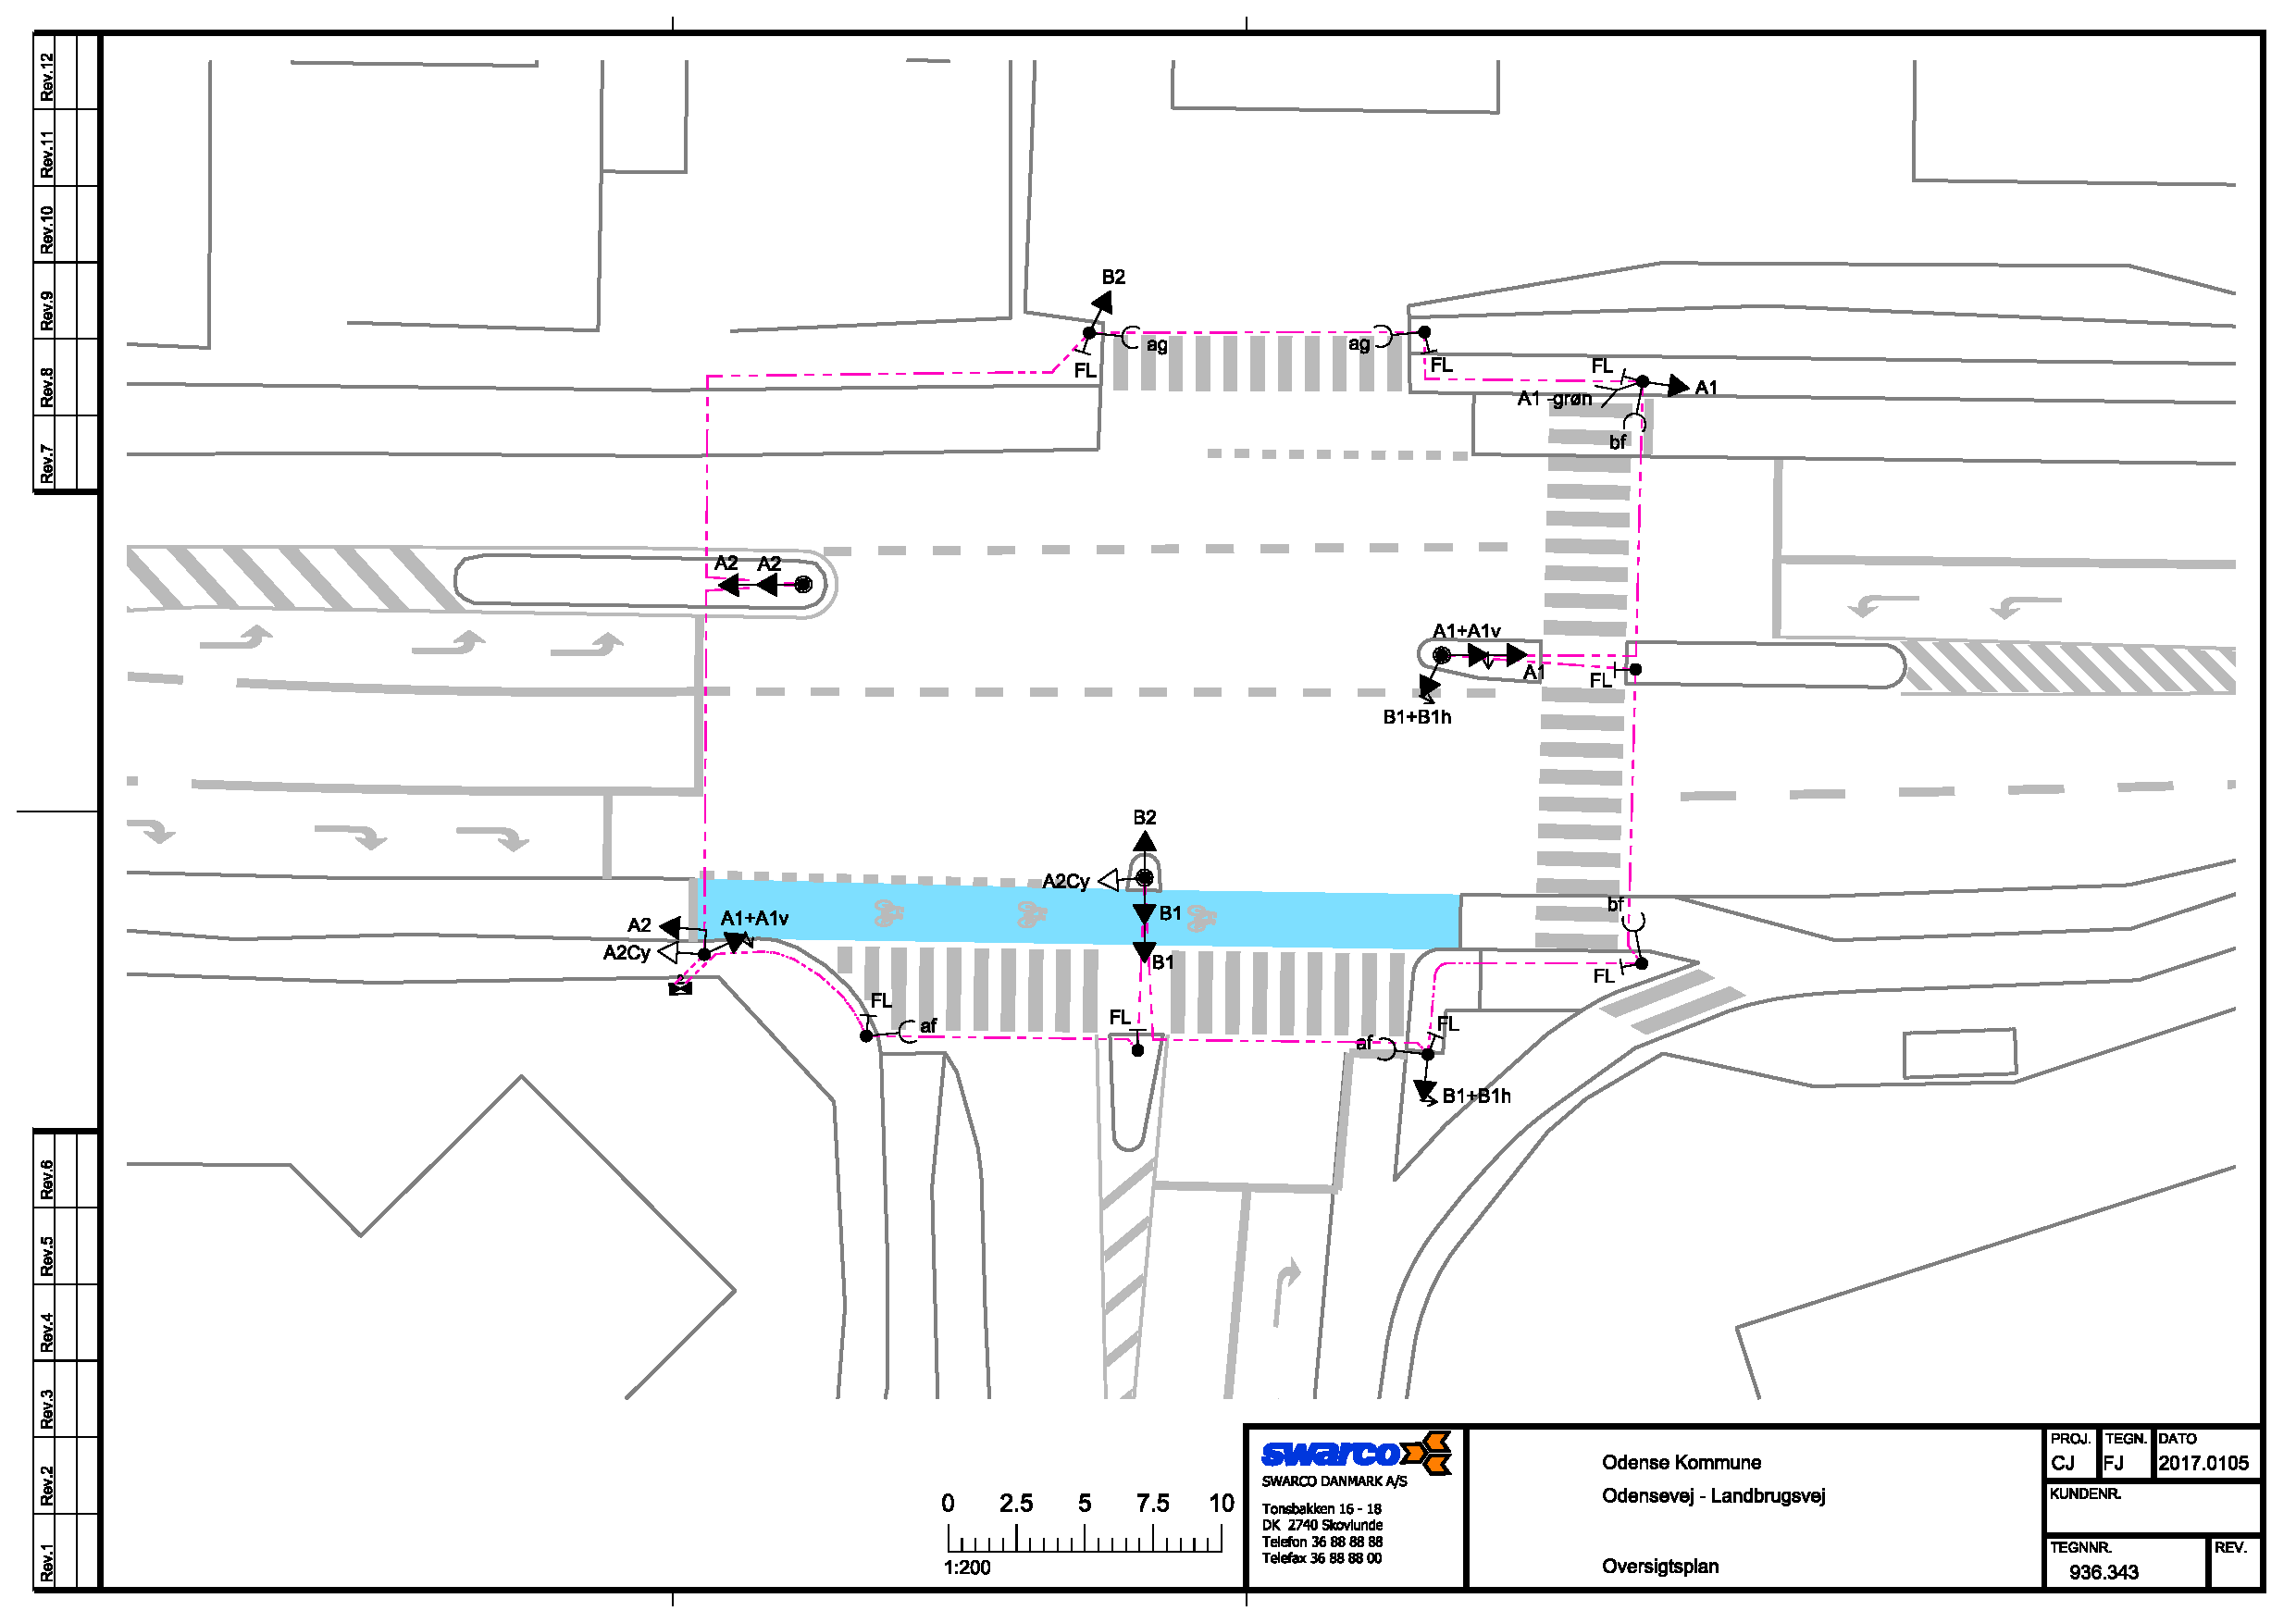
\includepdf[angle=270]{../include/Anl-427-traffic-light-movement.pdf}